\documentclass[12pt,a4paper]{article}

\usepackage[utf8]{inputenc}
\usepackage[a4paper,total={150mm,240mm}]{geometry}
\usepackage[american]{babel}

\usepackage{float}
\usepackage{babel}
\usepackage{amsmath}
\usepackage{tikz}
\usepackage{graphicx}
\usepackage{amssymb}
\usepackage{todonotes}


\usepackage{listings}
\definecolor{listingbg}{gray}{0.95}
\lstset{language=C++,basicstyle=\ttfamily\small,frame=single,backgroundcolor=\color{listingbg}}
% \lstset{language=C++, basicstyle=\ttfamily,
%   keywordstyle=\color{black}\bfseries, tabsize=4, stringstyle=\ttfamily,
%   commentstyle=\it, extendedchars=true, escapeinside={/*@}{@*/}}


\newcommand{\vx}{\vec x}
\newcommand{\grad}{\vec \nabla}
\newcommand{\wind}{\vec \beta}
\newcommand{\Laplace}{\Delta}
\newcommand{\mycomment}[1]{}


% Exercise stylesheet
\usepackage{exercise}

\title{\textbf{Exercises for Tutorial05}}
\subtitle{Adaptivity}
\exerciselabel{Exercise}


\begin{document}

\exerciseheader

\begin{Exercise}{Playing with Parameters of Adaptive the FE Algorithm}
The adaptive finite element algorithm is controlled by several parameters
which can be set in the ini-file.
Besides the polynomial degree these are:
\begin{itemize}
\item \lstinline{steps} : how many times the solve-- adapt cycle is executed.
\item \lstinline{uniformlevel} : how many times uniform mesh refinement is used before
adaptive refinement starts.
\item \lstinline{tol} : tolerance where the adaptive algorithm is stopped.
\item \lstinline{fraction} : Remember that the global error is estimated from element-wise
contributions: $$\gamma^2(u_h) = \sum_{T\in \mathcal{T}_h} \gamma_T^2(u_h).$$
The fraction parameter controls which elements are marked for refinement. More precisely,
the largest threshold $\gamma^\ast$ is determined such that
$$\sum_{\{T\in\mathcal{T}_h \,:\, \gamma_T(u_h)\geq\gamma^\ast\}} \gamma_T^2(u_h)
\geq \text{\lstinline{fraction}} \cdot \gamma^2(u_h). $$
If \lstinline{fraction} is set to zero no elements need to be refined, i.e. $\gamma^\ast=\infty$.
When \lstinline{fraction} is set to one then all elements need to be refined, i.e. $\gamma^\ast=0$.
A smaller \lstinline{fraction} parameter results in a more optimized mesh but needs more steps
and thus might be more expensive. If \lstinline{fraction} is chosen too large then almost
all elements are refined which might also be expensive, so there exists an (unknown) optimal
value for \lstinline{fraction}.
\end{itemize}
Carry out the following experiments:
\begin{enumerate}
\item Choose polynomial degree 1 and fix a tolerance, e.g. \lstinline{tol}=0.01.
Set \lstinline{steps} to a large number so that the algorithm is not stopped before the
tolerance is reached. Set \lstinline{uniformlevel} to zero. Now vary the \lstinline{fraction} parameter
and measure the execution time with
\begin{lstlisting}[basicstyle=\ttfamily\small,
frame=single,
backgroundcolor=\color{listingbg}]
$ time ./exercise05
\end{lstlisting}
\item Repeat the previous experiment with polynomial degrees two and three. Compare the optimal
meshes generated for the different polynomial degrees.
\item The idea of the heuristic refinement algorithm refining only the elements with the
largest contribution to the error is to \textit{equilibrate} the error. To check how well this
is achieved use the calculator filter in paraview to plot $\log(\gamma_T(u_h))$. Note that
the cell data exported by the (unchanged) code is $\gamma_T^2(u_h)$! Now check
the minimum and maximum error contributions. What happens directly at the singularity,
i.e. the point $(0,0)$?
\end{enumerate}
\end{Exercise}

\begin{Exercise}{Compute the True $L_2$-error}

To do this exercise we need some more background on PDELab grid functions.
The following code known from several tutorials by now
constructs a PDELab grid function object \lstinline{g}:
\begin{lstlisting}[basicstyle=\ttfamily\small,
frame=single,
backgroundcolor=\color{listingbg}]
Problem<RF> problem(eta);
auto glambda =
  [&](const auto& e, const auto& x){return problem.g(e,x);};
auto g = Dune::PDELab::makeGridFunctionFromCallable(gv,glambda);
\end{lstlisting}
Also the following code segement used in many tutorials constructs
a PDELab grid function object \lstinline{zdgf} from a grid function space and
a coefficient vector:
\begin{lstlisting}[basicstyle=\ttfamily\small,
frame=single,
backgroundcolor=\color{listingbg}]
typedef Dune::PDELab::DiscreteGridFunction<GFS,Z> ZDGF;
ZDGF zdgf(gfs,z);
\end{lstlisting}
PDELab grid functions can be evaluated in local coordinates given by an
element and a local coordinate within the corresponding reference element.
The result is stored in an additional argument passed by reference.
Here is a code segment doing the job:
\begin{lstlisting}[basicstyle=\ttfamily\small,
frame=single,
backgroundcolor=\color{listingbg}]
Dune::FieldVector<RF,1> truesolution(0.0);
g.evaluate(e,x,truesolution);
\end{lstlisting}
Here we assume that \lstinline{e} is an element and \lstinline{x} is a local coordinate.
The result is stored in a \lstinline{Dune::FieldVector} with one component of type
\lstinline{RF}. This allows also to return vector-valued results.

Now here are your tasks:
\begin{enumerate}
\item Extend the code in the file \lstinline{driver.hh} in \lstinline{tutorial05/exercise/src}
to provide a grid function that provides the error $u-u_h$. Note that the method \lstinline{g}
in the parameter class already returns the true solution (for $\eta=0$).
You can solve this task by writing a lambda function subtracting the values returned
by \lstinline{g.evaluate} and \lstinline{zdgf.evaluate}.
\item Compute the $L_2$-norm of the error, i.e. $\|u-u_h\|_0 = \sqrt{\int_\Omega
(u(x)-u_h(x))^2\,dx}$. This can be done by creating a grid function
with the squared error using \lstinline{Dune::PDELab::SqrGridFunctionAdapter}
from \lstinline{<dune/pdelab/function/sqr.hh>} and the function
\lstinline{Dune::PDELab::integrateGridFunction} contained in the header file
\lstinline{<dune/pdelab/common/functionutilities.hh>}.
Output the result to the console by writing in a single line a tag
like \lstinline{L2ERROR}, the number of degrees of freedom
using \lstinline{gfs.globalSize()} and the $L_2$-norm. This
lets you grep the results later for postprocessing.
\item Investigate the $L_2$-error for different polynomial degrees. Run the code
using different polynomial degrees and also uniform and adaptive (use your optimal
\lstinline{fraction}) refinement. Use \lstinline{gnuplot} to produce graphs such as
those in Figure \ref{Fig:L2}. An example gnuplot file \lstinline{plot.gp} is given.

The graph shows that for uniform refinement polynomial degree 2 is better than
polynomial degree 1 only by a constant factor. For adaptive refinement a better
convergence rate can be achieved. The plot also shows that for adaptive refinement
the optimal convergence rate can be recovered. For $P_1$ finite elements and fully regular
solution in $H^2(\Omega)$ the a-priori estimate for uniform refinement yields
$\|u-u_h\|_0\leq C h^2$. Expressing $h$ in terms of the number of degrees of freedom
$N$ yields $h\sim N^{-1/d}$, so $\|u-u_h\|_0\leq C h^2 \leq C' N^{-1}$ for $d=2$.
The curve $N^{-1}$ is shown for comparison in the plot. Clearly, the result for $P_1$ is parallel
to that line.
\item Optional: Also write the true error to the VTK output file.
\end{enumerate}

\end{Exercise}

\begin{figure}
\begin{center}
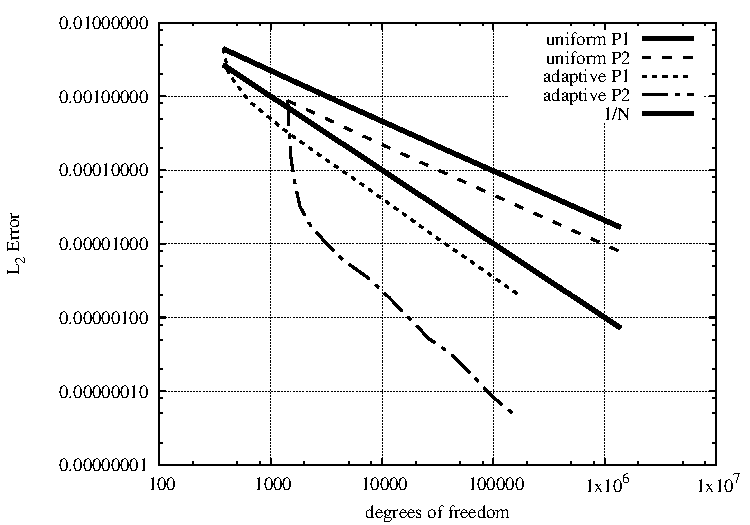
\includegraphics[width=\textwidth]{l2error}
\end{center}
\caption{$L_2$-error versus number of degrees of freedom for different polynomial degrees.}
\label{Fig:L2}
\end{figure}

\end{document}
